\section{Benchmark}

We perform quantig

\subsection{Dataset}

There are many publicly available datasets designed for tracking, however there is disagreement on how the data are stored. In order to facilitate the evaluation we collected the videos of different datasets and standardized how the data are stored. Each video is stored as a sequence of images while the ground truth, represented by an oriented bounding box, is saved in a comma separated value file where each row correspond to an image frame and contains 8 values representing the pairs x,y of each vertex of the box.  

\subsection{Evaluation Criteria}

In order to measure the
accuracy of our tracker we took into consideration many measures available in
the literature and decided to apply the widely used overlap measure:

\begin{equation}
	\Theta (b_{t}, b_{gt}) = \frac{b_{t} \cap b_{gt}}{b_{t} \cup b_{gt}}
\end{equation}

where \textit{$b_{t}$} is the bounding box estimated by our tracker and
\textit{$b_{gt}$} is the bounding box labeled manually and included in the
benchmark dataset. Computing the average per frame accuracy is not very
descriptive benchmark of the precision. I.e. an overall accuracy of 0.5 may
indicate either a very stable accuracy around that value or a tracker that is
very precise in part of the video sequence and non reliable in the
rest. Therefore, as suggested by other studies (e.g. \cite{nebehay14wccv}) we
define three thresholds $\Upsilon$ (0.25, 0.5, 0.75) that represent
requirements of low, medium and high tracking accuracy. The bounding box
\textit{$b_{t}$} is considered a true positive (TP) for a particular level of
accuracy $\Upsilon$ if:


\begin{equation}
\begin{cases}
b_{t} = TP  \text{ if } \Theta(b_{t}, b_{gt}) > \Upsilon \\
b_{t} = FP  \text{ otherwise }\\
\end{cases}
\end{equation}

we then calculate the overall accuracy of the tracker for each level of accuracy as:

\begin{equation}
\text{recall } = \frac{TP}{\text{TP } + \text{ FN}}
\end{equation}



\begin{figure}[t]
\centerline{% 
		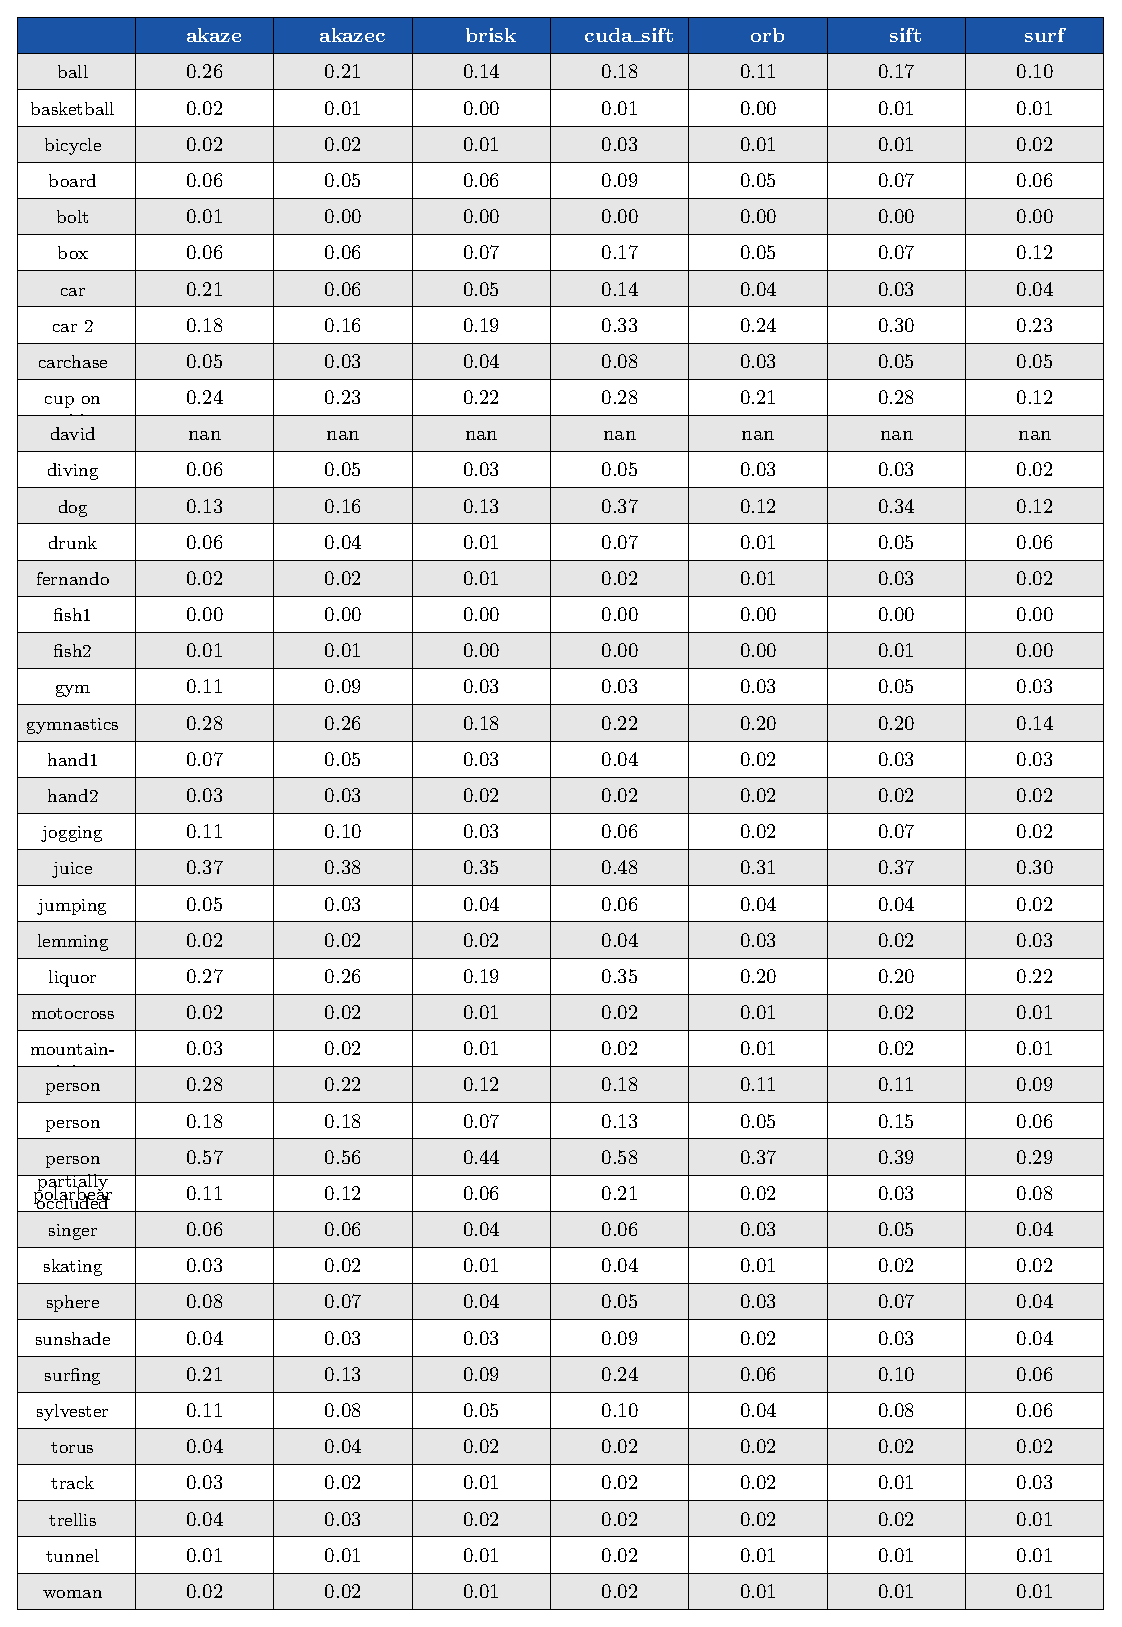
\includegraphics[width=0.98\linewidth]{tables/test.pdf}}
    \vspace{-2mm} 
	\caption{The figure shows the recall of our tracker with and
          without learning as the object undergoes motion (relative
          amount of motion is indicated with the continuous
          line). Recall is calculated according to three precision
          requirements (\ref{sec:bench}): low(blue), medium(red),
          high(green).}
	\label{fig:learnvsno}
\end{figure}

